\chapter{Concept}\label{cha:concept}
\section{Scenario: Mensa Community}
We illustrate the software system by considering a community of frequent canteen visitors. We will call this community the Mensa Community.
Although not a community of practice, the success principle can be applied to it, as members of the community share a common interest which they are passionate about: the food at their local canteen.
The success metrics for this community are based on the food quality and the activities and interest in their local canteen.
The members of the Mensa community are students and university employees.

The community has a hierarchical structure, consisting of different community levels.
In our case, the top level represents the community of all canteens in Germany.
The intermediate level represents the local Mensa community of a particular university.
The lowest level of the community represents a circle of friends, which frequent the canteen together. Note that members can belong to different circle of friends which means that communities can be overlapping.

Members of the community use community applications \footnote{\url{https://tech4comp.dbis.rwth-aachen.de/mensa/}}
\footnote{\url{https://monitor.tech4comp.dbis.rwth-aachen.de/}} to access information about the Mensa and their community.

embers of the community can interact with a chatbot, called \emph{mensabot}. The mensabot is modelled with  the Social Bot Framework. It can be accessed via the Slack chat in the Slack workspace of the community. Members can ask the bot about which food will be served on a given day.

As members of the Mensa community are very passionate about the food at the canteen, they can also use the bot to add a review of their meal.

Furthermore, members can query visualizations about the success of the community through the chat application. Those visualizations include current success metrics which were previously defined by members of the community. The metrics are defined using the MobSOS Evaluation center. The members can add measures to the success model of the community with the help of the bot.

\subsection{Use Cases}

\subsubsection{Get the menu for the canteen} A student, called Alice, wants to decide whether to go to the canteen on a given day. She opens the Slack app and asks the bot for the menu at the canteen on that day. The bot looks up the menu for that canteen and the resulting menu is then displayed inside the chat along with an average rating of reviews made by the community. The reviews help her to make a decision about which meal to choose.

\subsection{Setting a default city}
A university employee, called Bob asks the bot about the menu for a Mensa called "Mensa Academica". The bot finds two canteens matching that name. One is located in Aachen, while the other one is located in Leipzig. 
The bot asks Bob to clarify which canteen he meant by displaying both canteens in a list. Bob chooses the second item in the list and the bot returns the resulting menu.
The bot asks him if he wants to save the city, in which his canteen is based as his default city. This helps the bot to better identify the canteen on further requests.

\subsubsection{Adding a review} A student, called Charlie, just finished his meal at the canteen. To his surprise the food was better than expected. He decides to make a positive review using the mensabot. 
The bot will start a dialogue, by asking questions about the meal. Each question results in a data point for the review. The bot saves the review and displays the result in the chat

The user is asked if he wants to upload a photo of his meal. He chooses to do so. The final review is then added to the database and will be taken into consideration for further evaluation requests.


\subsubsection{Issuing a visualization request}
The student is still unsure on whether to go to the canteen. He asks the bot how popular a specific canteen is. The community had defined the popularity as a measure in the success model. The measure records the number of requests for the menu of that canteen and ranks it according to the other canteens.
The bot recognizes this as a predefined measure contained in the success model. He looks up information about the measure in the measure catalog. 

The measure contains all information about how to get the data and how to visualize it. This includes information about the database and the corresponding SQL query on that database. The bot transforms this information into a GraphQL request and sends it to the GraphQL interface of the CCA system. The GraphQL server returns the appropriate data.

The bot then visualizes this data and displays the  resulting visualization inside the chat.
After the user has seen how good the food is, he is asked by the bot, whether he will go to the canteen. He tells the bot that he will go.

\subsubsection{Success Awareness} Students in the Mensa community are aware that the success of their community depends on the active participation of its members. They are discussing about the success of the community inside a group chat. They want to know how active the members of the community are. A student mentions the bot, which is a member of the chat group. They tell it to visualize the average time, that a user is interacting with the service. The bot recognizes this as a measure and runs a predefined query. The resulting data is visualized in the group chat.

\subsubsection{Success modelling} The students see a trend in the visualization, which indicates that there are less people using the bot.
The students blame the Corona virus for this negative trend as the canteen can only be used as takeout. Furthermore, a lot of students returned to their hometowns.
The students want to verify that the lack of activities is indeed due to Corona virus and not due to decreasing food quality.
They ask the bot to update the success model of their community.
They add a measure which models the average stars of reviews over time.
After visualizing the new metric, they observe that the average stars have remained more or less constant over time.

The students are asked to add a comment to the change, so that members of the community can understand the reason for the change at a later date.


\subsubsection{Modifying a review} A user just added a review to the database. He realizes that he forgot to mention the excellent quality of the fries. 
He asks the bot if he can still update his review. The bot will ask the user the same questions and afterwards update the entry in the database with the new review.

\subsubsection{Evaluating the service} A user, which has been using the service for some time, is asked questions about the quality of the service. Such questions include things like how satisfied they are with different aspects of the service, or how likely it is, that they would recommend the service to a colleague.

\subsubsection{Adding a new database} Core members and moderators of the community can add a new source of information by adding a new database to the system. This can be done with the help of the GUI of the CCA system and the MobSOS query visualization service.
The moderators are aware that many members of the community also add reviews on sites like Google reviews. 
They add a Mediabase containing reviews collected by crawlers from sites like Google Reviews.

\subsubsection{Visualizations of multiple databases} Multiple databases can exist in a system. Apart from the reviews, which were added by chat, other reviews about overall user satisfaction are also collected with the help of crawlers. A student request a visualization of a metric which represents the overall success of the community.
The data is aggregated from different sources, like reviews on Facebook, Google, which are stored in the Mediabase, and reviews which were made inside the las2peer system. 
The resulting visualization contains results from all databases, to give an overview on how popular the specific canteen really is.

\begin{figure}
    \centering
    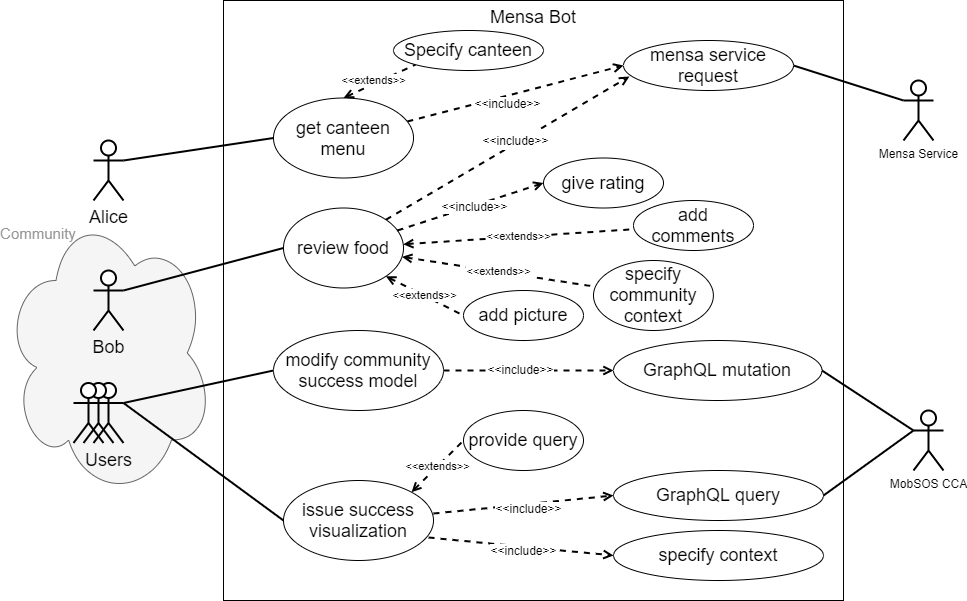
\includegraphics[width=0.8\linewidth]{concept/usecase.png}
    \caption{Use case diagram for the Chatbot}
\end{figure}

\section{Requirements}
The requirements are derived from the use case. We distinguish between functional and non-functional requirements.
\subsection{Functional Requirements}

\subsubsection{Retrieving Data from GraphQL API}
The system needs to be able to make queries to the GraphQL API, to get data, which will be used for the visualization of success metrics. The GraphQL API  for the Continuous Community Analytics systems provides data from different data sources, such as a las2peer database, a Mediabase with data, which is collected from outside the las2peer system and a database, which contains service logs.

\subsubsection{Get Menu for the Canteen} The bot needs to be able to get the menu for a specific canteen for the given day and display it inside the chat as a list of text items. The service should be able to use the OpenMensa API \footnotemark in order to get the menu for canteens all over Germany.

\footnotetext{\href{https://doc.openmensa.org/api/v2/}{https://doc.openmensa.org/api/v2/}}

\subsubsection{Enter Review Context} The bot should be able to recognize, if a user wants to start a review. This can be done with the help of intent recognition from a RASA server.

\subsubsection{Group Chats} Users should be able to add a bot to a group chat.

\subsubsection{Listen for Mentions} Inside a group chat, the bot should only respond to messages which specifically mentioned the bot. This is important to prevent the bot from spamming the chat.

% \subsubsection{Create new templates} The bot needs to be able to create visualization-request templates and add them to the database.

\subsubsection{Use Google Charts API} The data which has been retrieved from the GraphQL API needs to be passed to the Google Charts API to create a visualization. The resulting visualization should be a picture, so that it can be represented inside a chat. The visualization can be rendered by using an HTML image generator.

\subsubsection{Cope with spelling mistakes} The bot should be able to understand the user, even if they made a spelling mistake.

\subsection{Non-Functional Requirements}

\subsubsection{Usability} The bot should be easy to use. Non-trained users should be able to interact with the bot with ease.

\subsubsection{UI optimization} The bot should be designed, for chats which will mainly run on mobile devices. As such, visualizations should be easy to read even on small devices.

\subsubsection{Compatibility} The bot should be extensible to any chat platform, which allows the use of bots.

\section{System overview}


\begin{figure}[h]
    \centering
    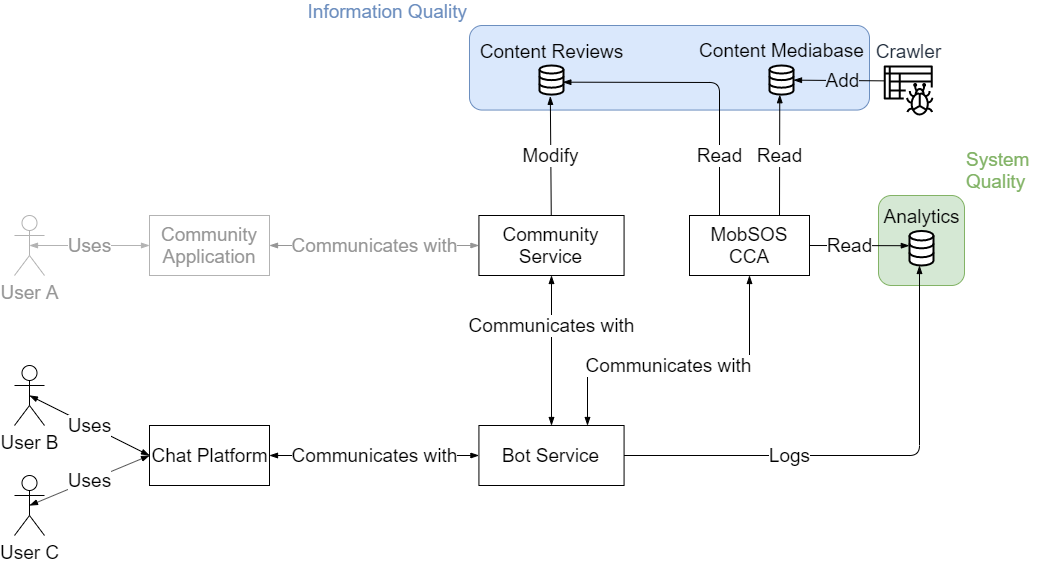
\includegraphics[width=\linewidth]{realization/Component_Diagramm.png}
    \caption{System overview}
    \label{fig:sytsemOverview}
\end{figure}

Figure \ref{fig:sytsemOverview} shows how the \emph{Bot Service} can be integrated into an existing community information system. Users communicate with the \emph{Chat Platform}, which transmits requests to the Bot Service.

The Bot Service communicates with the \emph{Community Service} in order to provide users the same, or similar, information as an existing \emph{Community Application}. The bot service also communicates with the \emph{MobSOS CCA} system in order to retrieve success visualizations and display them as charts on the Chat Platform. Users can also use the chat to model success queries and modify the existing success model.

Both the community service and the bot service log request, which are stored in a database representing the \emph{System Quality} dimension of the MobSOS success model. Those logs can be retrieved by the MobSOS CCA system. Furthermore, the MobSOS CCA system also has access to a variety of content databases which represent the \emph{Information Quality} dimension of the MobSOS success model.